This subsection shows the avg. of \emph{User Profile 1}'s results, the avg. of \emph{User Profile 2}'s results and the avg. between the two. We have chosen to give you also the separates view of the two groups to better understand how different segments react to the same tasks.

\subsection{Avg. User Profile 1}
{
\captionof{table}{Avg per task}
\centering
\begin{tabular}{lllllll} 
	\toprule
	\textbf{Scenario } & \textbf{Task} & \begin{tabular}[c]{@{}l@{}}\textbf{Execution}\\\textbf{Time (s)}\end{tabular} & 			\textbf{Success} & \begin{tabular}[c]{@{}l@{}}\textbf{Perceived}\\\textbf{Difficulty}\end{tabular} & \textbf{Errors} & 			\textbf{Satisfaction}  \\
	Scenario 1 & 1             & 9,4                 	& 100\%          	& 0					& 0					& 4,8           	                                                                 \\
	Scenario 1 & 2             & 8,6                   	& 100\%          	& 0					& 0					& 5                                                                                \\
	Scenario 1 & 3             & 15,2                 	& 100\%          	& 0,2				& 0,2				& 4,8                                                                               \\
	Scenario 2 & 1             & 8,8                 	& 100\%          	& 0,2				& 0,2				& 4,6                                                                              \\
	Scenario 2 & 2             & 36,4                   	& 100\%        	& 0					& 0,2				& 4,8                                                                                \\
	Scenario 2 & 3             & 46                 	& 100\%          	& 0,4				& 0,6				& 4,8                                                                                \\
	Scenario 3 & 1             & 8,2                 	& 100\%         	& 0					& 0					& 4,6                                                                                \\
	Scenario 3 & 2             & 11,2                 	& 100\%          	& 0					& 0					& 4,8                                                                                \\
	Scenario 3 & 3             & 18,6                	& 100\%          	& 0,4				& 0,2				& 4,6                                                                                 \\
\bottomrule
\end{tabular}

\vspace{1cm}
}It is possibile to see that, for this segment, the tasks 2 and 3 of scenario 2 has been the most complex and difficult and it can be seen becase the execution time is the heigher as the number of mistakes made and as the perceived difficulty. Even though the results into scenario 2 aren't that good, the satisfaction is high because they said that the problems they faced where related to the language. They suggested to add the multi-language feature in other to avoid the language barrier.\\
The next figure has the aim to show the avg between all scenarios.

\begin{figure}[h!]
	\centering
	\begin{minipage}[b]{1\textwidth}
    		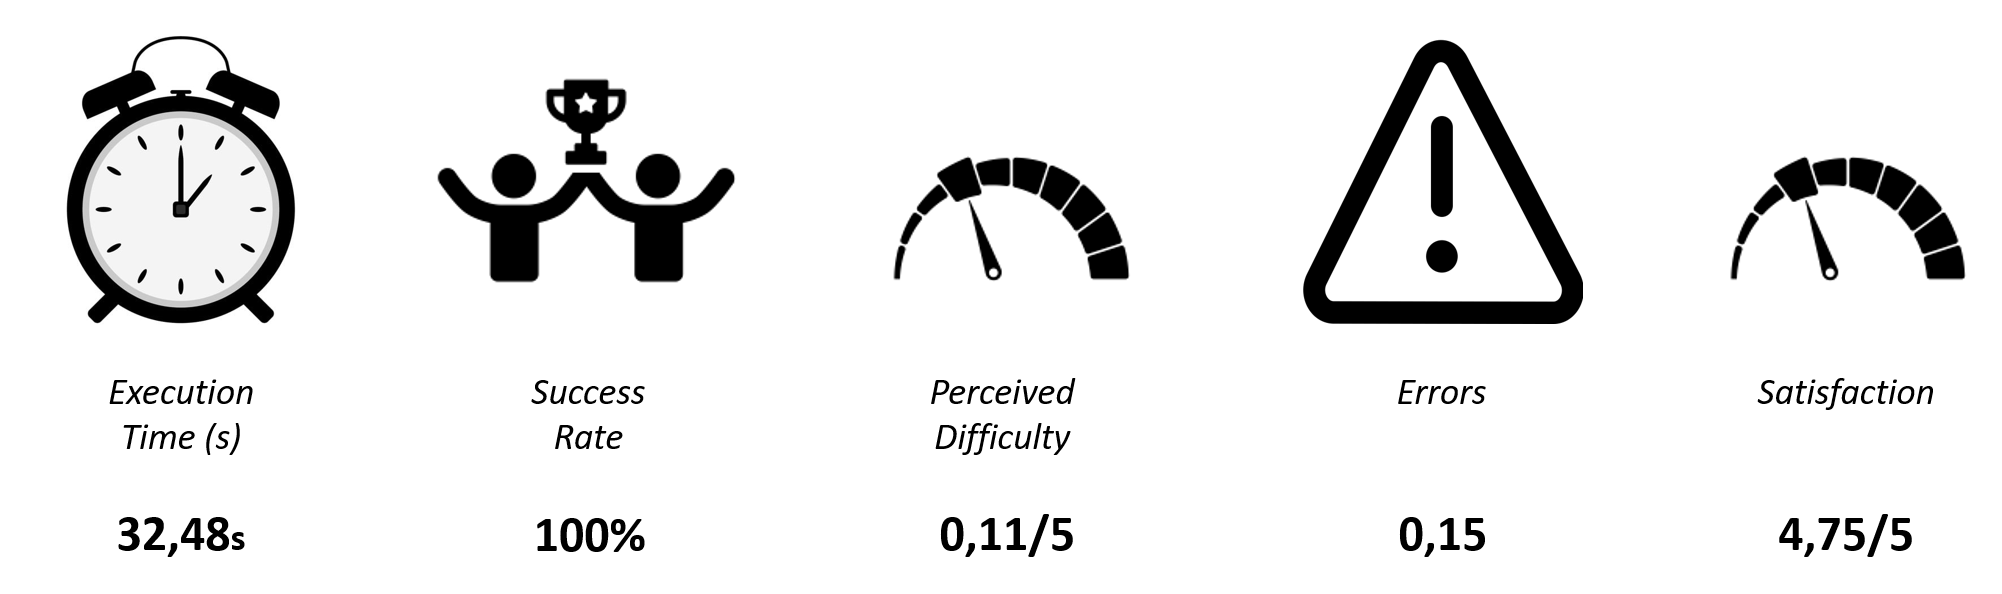
\includegraphics[width=\textwidth]{./assets/avg-1.png}
		\caption{\emph{Total Avg. user profile 1}: the avg obtained here is between the 3 scenarios }
	\end{minipage}
\end{figure}
\FloatBarrier


\subsection{Avg. User Profile 2}
{
\captionof{table}{Avg per task}
\centering
\begin{tabular}{lllllll} 
	\toprule
	\textbf{Scenario } & \textbf{Task} & \begin{tabular}[c]{@{}l@{}}\textbf{Execution}\\\textbf{Time (s)}\end{tabular} & 			\textbf{Success} & \begin{tabular}[c]{@{}l@{}}\textbf{Perceived}\\\textbf{Difficulty}\end{tabular} & \textbf{Errors} & 			\textbf{Satisfaction}  \\
	Scenario 1 & 1             & 15,25                 	& 100\%          	& 0					& 0					& 5           	                                                                 \\
	Scenario 1 & 2             & 8                   	& 100\%          	& 0					& 0					& 5                                                                                \\
	Scenario 1 & 3             & 19                 	& 100\%          	& 1,5				& 1,75				& 3,75                                                                               \\
	Scenario 2 & 1             & 10,75                 	& 100\%          	& 0,25				& 0,25				& 4,75                                                                              \\
	Scenario 2 & 2             & 8,5                   	& 100\%        	& 0					& 0					& 5                                                                                \\
	Scenario 2 & 3             & 9,75                 	& 100\%          	& 1					& 0,5				& 4                                                                                \\
	Scenario 3 & 1             & 15,25                 	& 100\%         	& 0					& 0					& 5                                                                                \\
	Scenario 3 & 2             & 15                 	& 100\%          	& 0					& 0					& 5                                                                                \\
	Scenario 3 & 3             & 14,5                	& 100\%          	& 0,25				& 0					& 4,5                                                                                 \\
\bottomrule
\end{tabular}

\vspace{1cm}
}It is possibile to see that for this segment the 3 task of scenario 1 has been the most complex and difficult and it can be seen becase the execution time is the heigher as the number of mistakes made and the satisfaction rate is the lower one. \\
The next figure has the aim to show the avg between all scenarios.

\begin{figure}[h!]
	\centering
	\begin{minipage}[b]{1\textwidth}
    		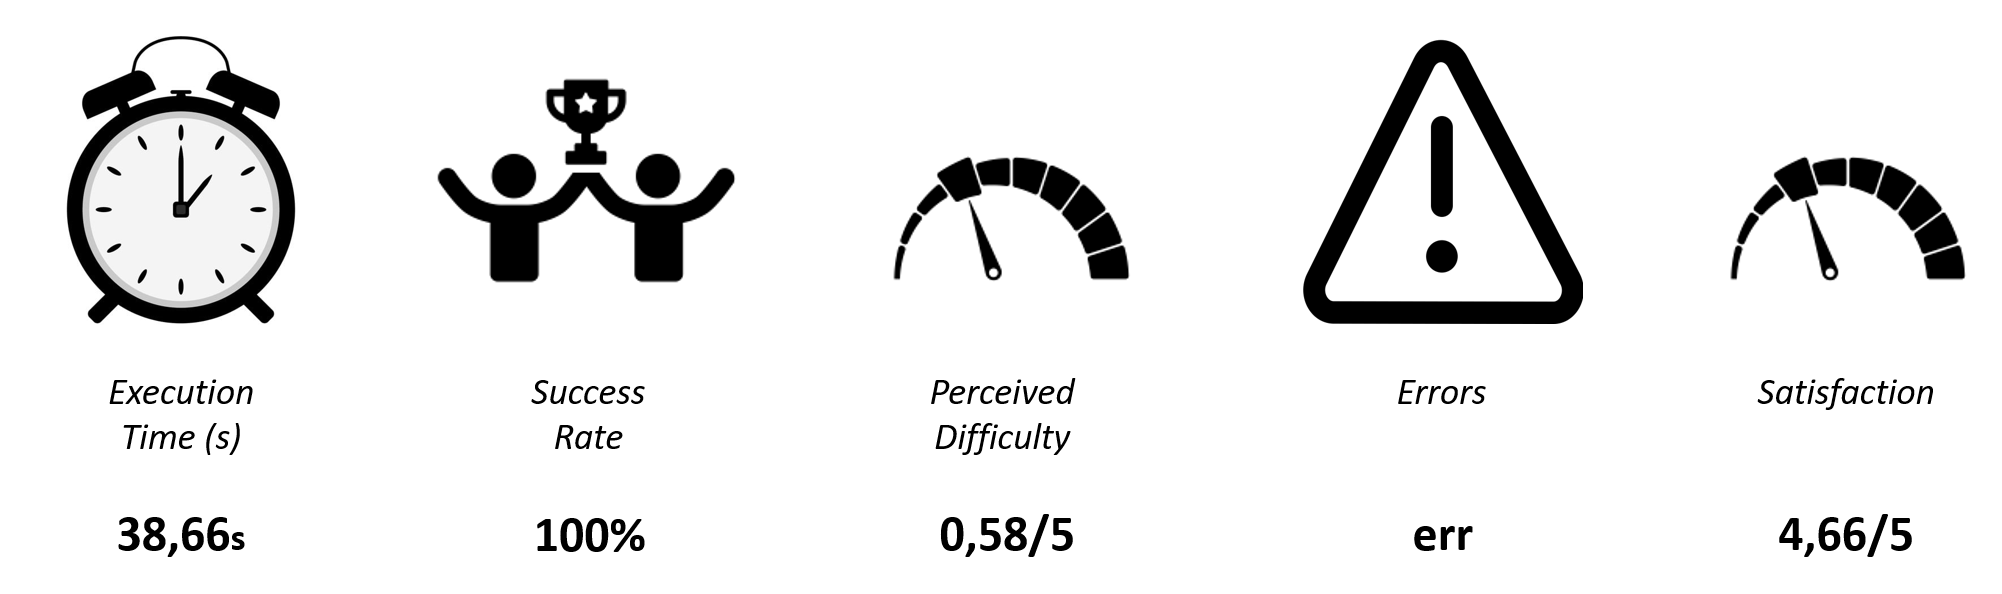
\includegraphics[width=\textwidth]{./assets/avg-2.png}
		\caption{\emph{Total Avg. user profile 2}: the avg obtained here is between the 3 scenarios }
	\end{minipage}
\end{figure}
\FloatBarrier


\subsection{Total Avg.}
We have seen that there isn't a big difference between the results obtained by the 2 segments and we have also noticed that the avg of segment 2 is always higher than the avg obtain by segment 1 except for the satisfaction, which is lower. The next figure wrap up the results of the two,  in order to give a general final picture of scenarios. execution.
\begin{figure}[h!]
	\centering
	\begin{minipage}[b]{1\textwidth}
    		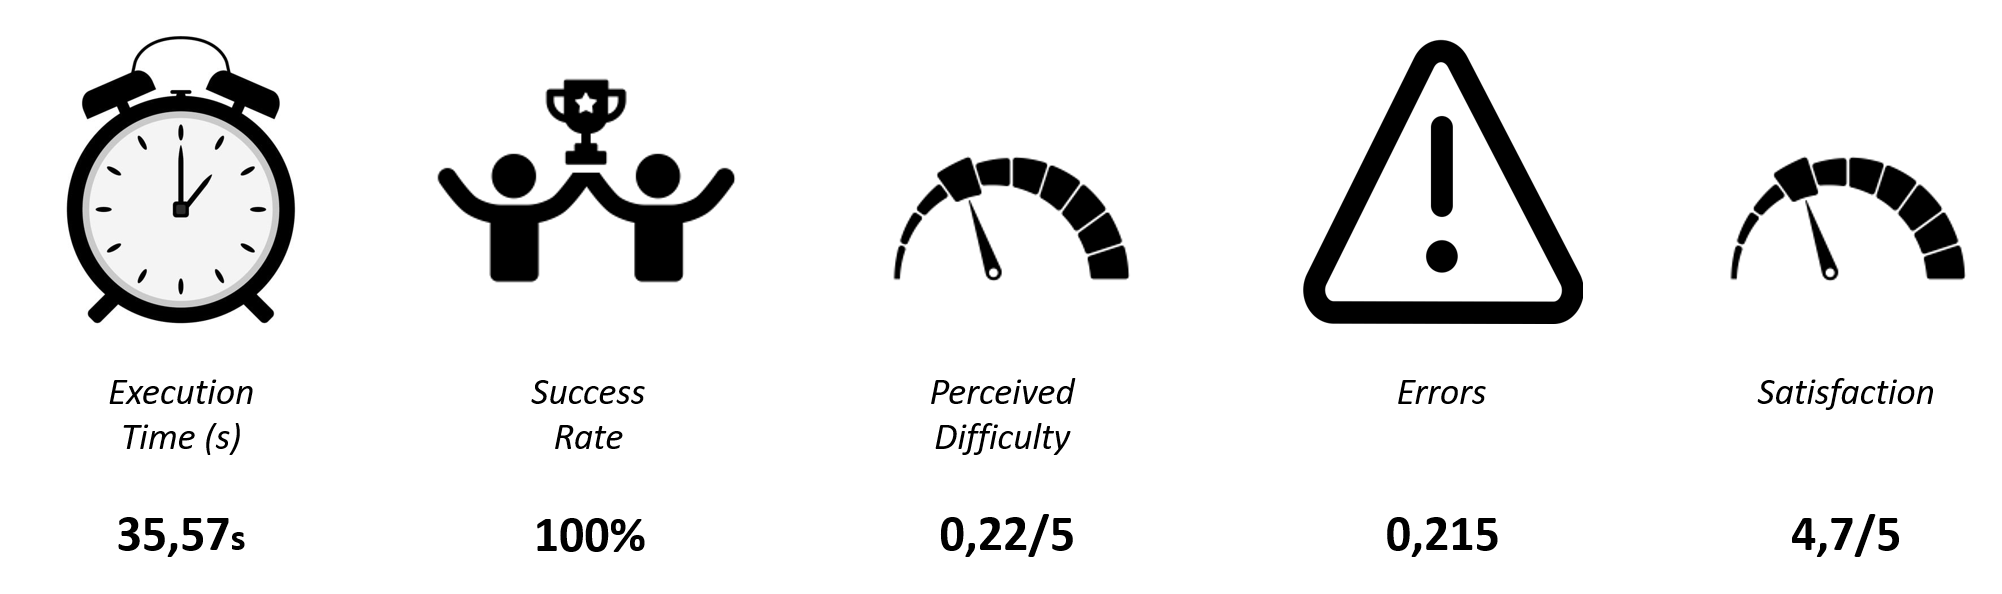
\includegraphics[width=\textwidth]{./assets/avg-tot.png}
		\caption{\emph{Total Avg.}: the avg obtained here is between the 2 segments}
	\end{minipage}
\end{figure}
\FloatBarrier

\subsection{Survey results}
This section has the aim to show the avg result of each survey question and how the answers are divided between the different values.

\begin{figure}[h!]
	\centering
	\begin{minipage}[b]{1\textwidth}
    		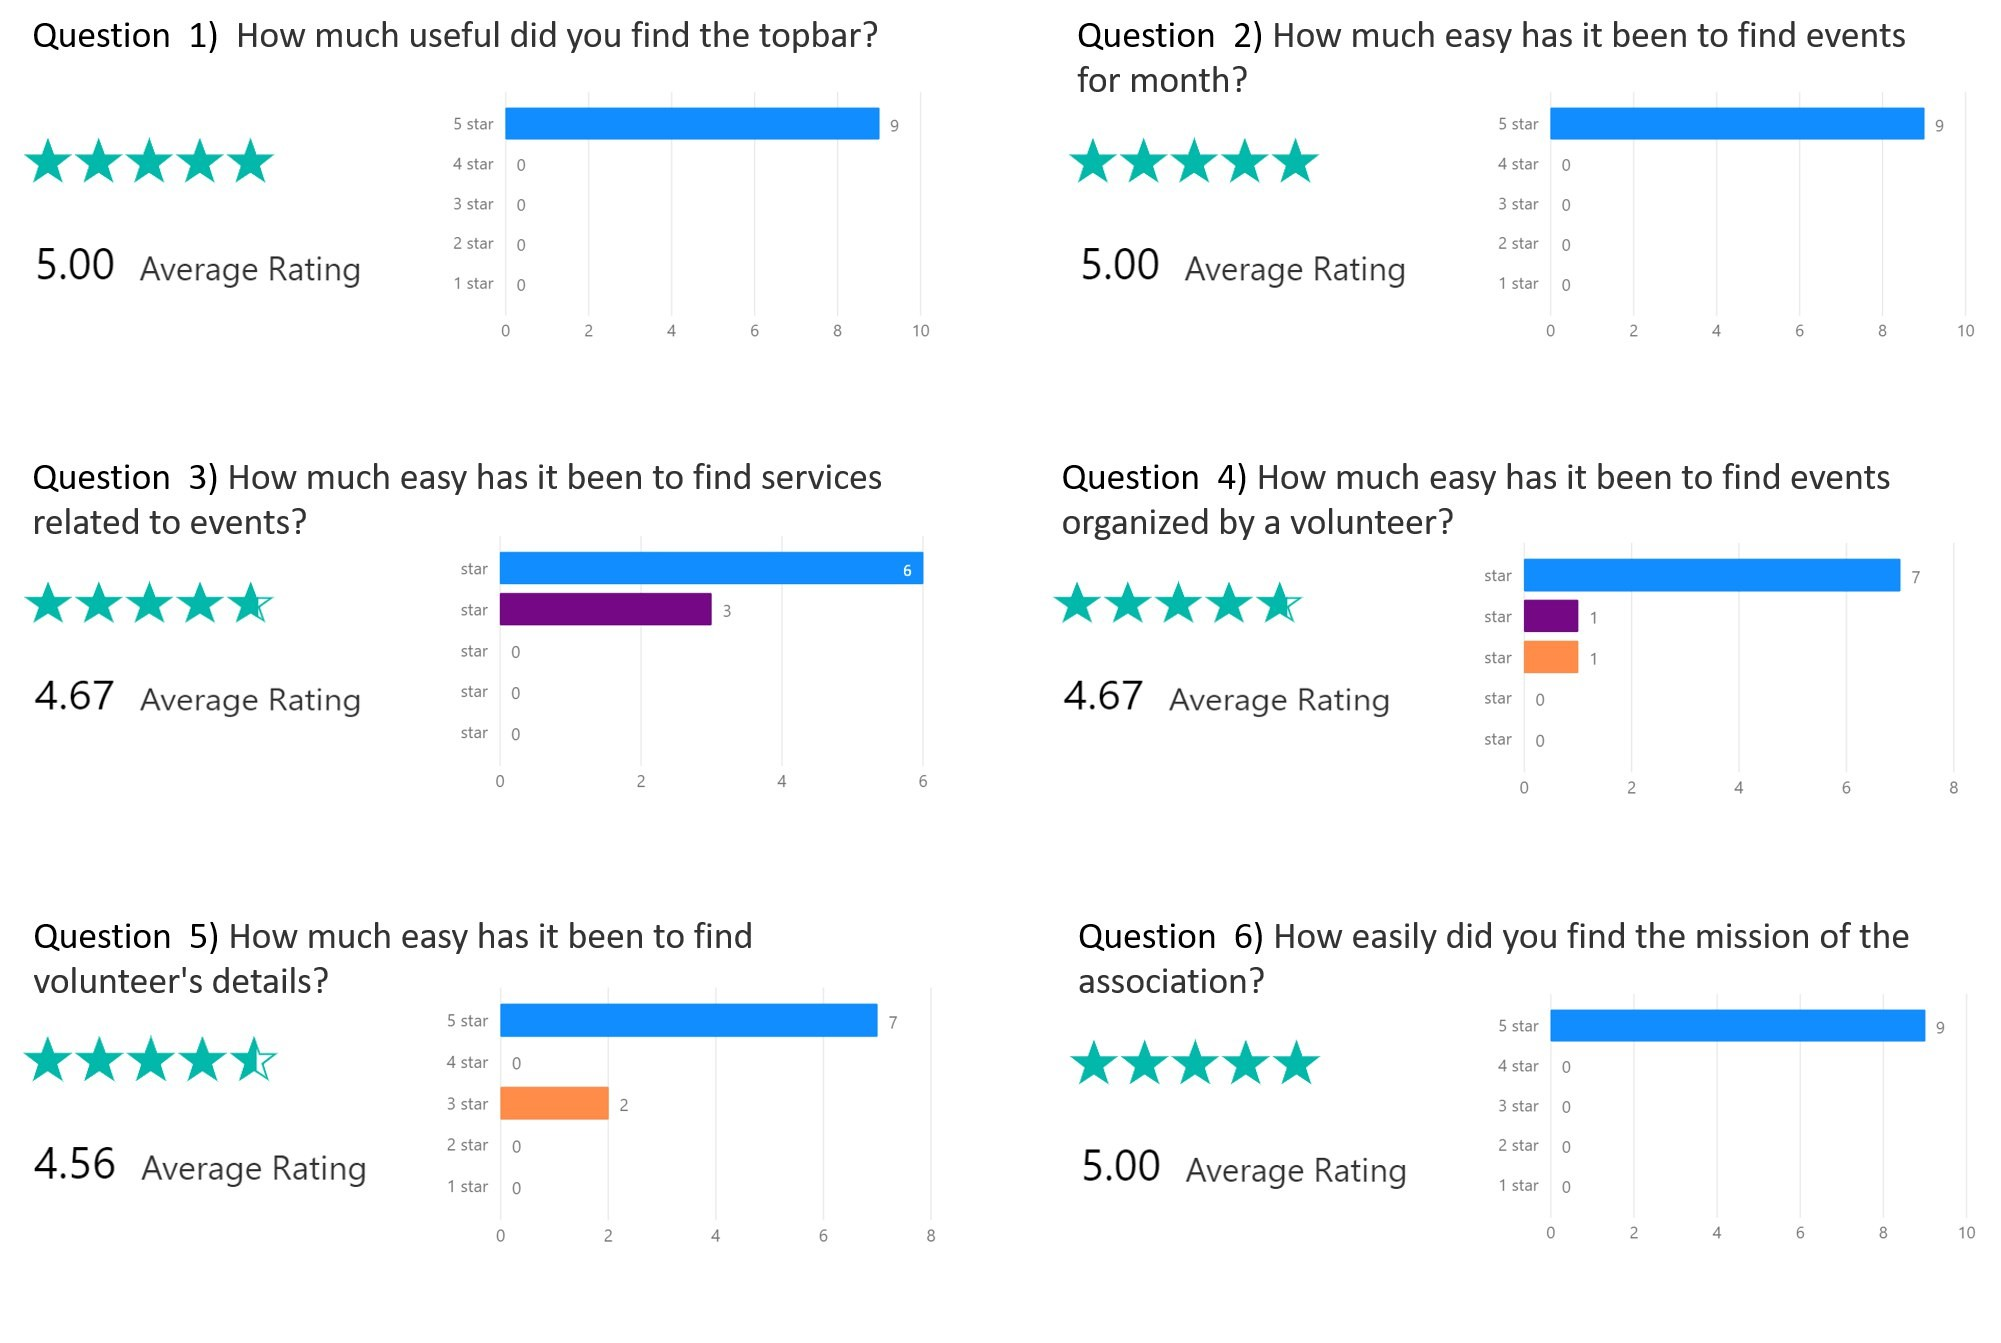
\includegraphics[width=\textwidth]{./assets/survey-results.jpg}
		\caption{Survey answers results}
	\end{minipage}
\end{figure}
\FloatBarrier
\begin{figure}[h!]
	\centering
	\begin{minipage}[b]{1\textwidth}
    		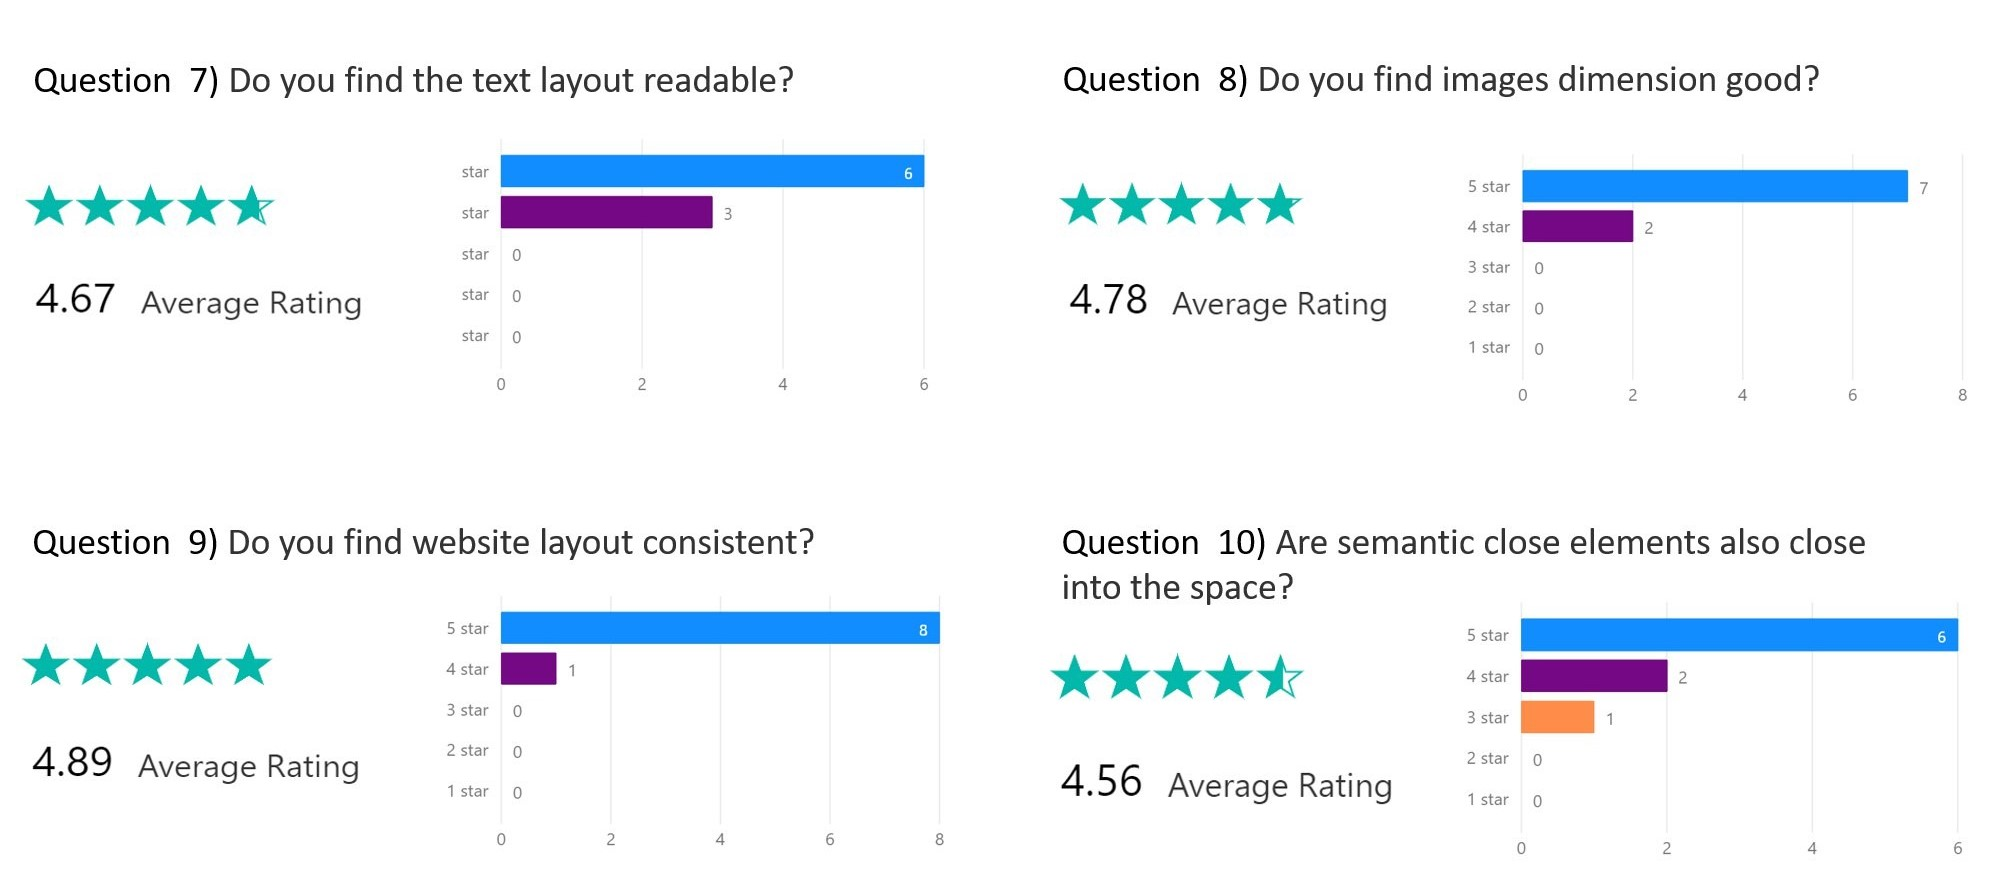
\includegraphics[width=\textwidth]{./assets/survey-results-1.jpg}
		\caption{Survey answers results}
	\end{minipage}
\end{figure}
\FloatBarrier
